\documentclass[aspectratio=169,11pt]{beamer}

% ================================================================
% "TABIIY TILNI QAYTA ISHLASH" KURSI
% MA'RUZA 14 --- RAG va vektor ma'lumotlar bazalari
%              (d14_rag.tex)
% Arxetiplar: [A][B][C][D][E] + 4 tsikl [F][G][H][I][J][K][L] +
%             [M][N][O][P][Q][R] + ilova [S]
% Rendered slayd soni: ~47 (4-haftaning RAG ma'ruzasi; L1-L13 chuqurligi)
% Qulflangan [I2]: RAG prompt = 700 token; 700/128000 < 1%; retrieved_docs = 3
%   --- P14 (Day 15) birinchi assert manbayi (course_map hand_example).
% MUHIM ARK: L13 fine-tuning bilimni sozlaydi -> L14 RAG yangi faktni qidirib keltiradi.
% ================================================================

% ================================================================
% RANGLAR  (asl fayldan o'zgarishsiz)
% ================================================================
\definecolor{cnublue}{rgb}{0.07,0.14,0.62}
\definecolor{cnubluelight}{rgb}{0.18,0.30,0.72}
\definecolor{cnubluebg}{rgb}{0.90,0.92,0.97}
\definecolor{deepblue}{rgb}{0.07,0.14,0.62}
\definecolor{deepred}{rgb}{0.60,0.00,0.00}
\definecolor{deepgreen}{rgb}{0.00,0.45,0.00}
\definecolor{halfgray}{gray}{0.55}

% ================================================================
% BEAMER MAVZU --- Boadilla + maxsus footer  (asl fayldan o'zgarishsiz)
% ================================================================
\usetheme{Boadilla}

\setbeamercolor{structure}{fg=cnublue}
\setbeamercolor{frametitle}{bg=cnublue,fg=white}
\setbeamercolor{title}{bg=cnublue,fg=white}
\setbeamercolor{block title}{bg=cnublue,fg=white}
\setbeamercolor{block body}{bg=cnubluebg,fg=black}
\setbeamercolor{alerted text}{fg=deepred}
\setbeamercolor{author in head/foot}{bg=cnubluelight,fg=white}
\setbeamercolor{section in head/foot}{bg=cnublue,fg=white}
\setbeamercolor{page number in head/foot}{bg=cnubluelight,fg=white}

\setbeamertemplate{mini frame}{}
\setbeamertemplate{mini frame in current section}{}
\setbeamertemplate{mini frame in current subsection}{}
\setbeamertemplate{headline}{}
\setbeamertemplate{navigation symbols}{}

\setbeamertemplate{footline}{%
  \leavevmode%
  \hbox{%
    \begin{beamercolorbox}[wd=0.17\paperwidth,ht=2.5ex,dp=1.25ex,leftskip=0.5em]{author in head/foot}%
      \usebeamerfont{author in head/foot}\scriptsize\insertshortauthor%
    \end{beamercolorbox}%
    \begin{beamercolorbox}[wd=0.69\paperwidth,ht=2.5ex,dp=1.25ex,center]{section in head/foot}%
      \usebeamerfont{section in head/foot}%
      \scriptsize\insertsectionnavigationhorizontal{0.69\paperwidth}{}{}%
    \end{beamercolorbox}%
    \begin{beamercolorbox}[wd=0.14\paperwidth,ht=2.5ex,dp=1.25ex,rightskip=0.5em]{page number in head/foot}%
      \hfill\scriptsize\color{white}%
      \insertframenumber{}/\inserttotalframenumber%
    \end{beamercolorbox}%
  }%
  \vskip0pt%
}

% ================================================================
% PAKETLAR  (asl fayldan o'zgarishsiz)
% ================================================================
\usepackage[utf8]{inputenc}
\usepackage[T1]{fontenc}
\usepackage{lmodern}
\usepackage{amsmath,amssymb}
\usepackage{booktabs}
\usepackage{xcolor}
\usepackage{listings}
\lstset{
    language=Python,
    basicstyle=\ttfamily\scriptsize,
    keywordstyle=\bfseries\color{deepblue},
    emphstyle=\ttfamily\color{deepred},
    stringstyle=\color{deepgreen},
    commentstyle=\itshape\color{halfgray},
    numbers=left,
    numberstyle=\scriptsize\color{halfgray},
    rulesepcolor=\color{cnublue!30},
    frame=shadowbox,
    breaklines=true,
    showstringspaces=false,
    tabsize=2
}
\usepackage{tcolorbox}
\tcbuselibrary{skins}
\tcbset{
  defbox/.style={colback=cnubluebg,colframe=cnublue,
                 fonttitle=\small\bfseries\color{white},
                 attach boxed title to top left={yshift=-2mm,xshift=4mm},
                 boxed title style={colback=cnublue,colframe=cnublue}},
  warnbox/.style={colback=orange!8,colframe=orange!70!black,
                  fonttitle=\small\bfseries},
  okbox/.style={colback=green!7,colframe=green!55!black,
                fonttitle=\small\bfseries}
}
\usepackage{tikz}
\usetikzlibrary{arrows.meta,positioning}

% ================================================================
% QO'SHIMCHALAR  (asl fayldan o'zgarishsiz)
% ================================================================
\AtBeginSection[]{%
  \begin{frame}{Prezentatsiya rejasi}
    \tableofcontents[currentsection]
  \end{frame}}

\newcommand{\bunda}[1]{{\small\textbf{bunda:}\; #1}}
\newcommand{\bajarildi}{{\color{deepgreen}\large$\checkmark$}\;}

% ================================================================
% METAMA'LUMOT
% ================================================================
\title[RAG]{RAG va vektor ma'lumotlar bazalari}
\subtitle{Tabiiy tilni qayta ishlash --- 14-ma'ruza}
\author[A.A.\,Abdulali]{A.A.\,Abdulali}
\date{7-iyul 2026}
\institute{11:00--12:20 \quad$\cdot$\quad mavzu \textnumero{}14}

% ================================================================
\begin{document}
% ================================================================

% ----------------------------------------------------------------
% [A] TITUL
% ----------------------------------------------------------------
\maketitle

% ================================================================
\section[Kirish]{Kirish: modelga yangi bilimni qidirib beramiz}
% ================================================================

% ----------------------------------------------------------------
% [B] TAKRORLASH: L13 va bugungi P13
% ----------------------------------------------------------------
\begin{frame}{Takrorlash: o'tgan darsdan ikki savol}
  \begin{columns}[T]
    \begin{column}{0.49\textwidth}
      \begin{tcolorbox}[warnbox,title=1-savol]
        \small
        L13 da fine-tuning modelni vazifaga sozladi. Fine-tuning modelga
        \textbf{yangi faktlar} (masalan, kechagi yangilik) ni qo'sha oladimi?
      \end{tcolorbox}
    \end{column}
    \begin{column}{0.49\textwidth}
      \begin{tcolorbox}[warnbox,title=2-savol]
        \small
        LLM bilmagan savolga duch kelsa nima qiladi --- "bilmayman" deydimi
        yoki ishonch bilan xato javob beradimi?
      \end{tcolorbox}
    \end{column}
  \end{columns}
  \pause
  \vspace{4pt}
  \begin{columns}[T]
    \begin{column}{0.49\textwidth}
      \begin{tcolorbox}[okbox,title=1-javob]
        \small
        Yo'q --- fine-tuning bilimni \textbf{sozlaydi}, yangi faktni arzon
        qo'shmaydi. Har yangilik uchun qayta o'qitish qimmat.
      \end{tcolorbox}
    \end{column}
    \begin{column}{0.49\textwidth}
      \begin{tcolorbox}[okbox,title=2-javob]
        \small
        Ko'pincha ishonch bilan \textbf{gallyutsinatsiya} qiladi. Yechim:
        tashqi manbadan qidirib, javobni unga tayantirish --- \textbf{RAG}.
      \end{tcolorbox}
    \end{column}
  \end{columns}
\end{frame}

% ----------------------------------------------------------------
% [C] MAQSADLAR
% ----------------------------------------------------------------
\begin{frame}{Siz bugungi dars oxirida quyidagilarni bajara olasiz:}
  \begin{enumerate}\setlength\itemsep{6pt}
    \item \textbf{Tushuntira olasiz:} LLM cheklovlari (gallyutsinatsiya, bilim
          eskirishi) va RAG nega yordam berishini.
    \item \textbf{Hisoblay olasiz:} RAG prompt token byudjetini --- 3 chunk
          $+$ instruction $= 700$ token ($<1\%$ kontekst oynasi).
    \item \textbf{Tushuntira olasiz:} vektor embeddinglar bilan semantik
          qidiruvni (kosinus o'xshashlik, top-k).
    \item \textbf{Tushuntira olasiz:} vektor ma'lumotlar bazalari (Pinecone,
          Weaviate) RAG dagi rolini.
  \end{enumerate}
  \vspace{4pt}
  \begin{tcolorbox}[defbox,title=Oldindan talab]
    \footnotesize
    L13 dan: fine-tuning. L3/L6 dan: embedding, kosinus o'xshashlik. L4 dan:
    o'xshashlik qidiruvi (LSH). Matematikadan: skalyar ko'paytma, ulush.
  \end{tcolorbox}
\end{frame}

% ----------------------------------------------------------------
% [D] REJA
% ----------------------------------------------------------------
\begin{frame}{Bugungi dars rejasi:}
  \begin{center}
  \small
  \begin{tabular}{c p{5.2cm} c p{3.0cm}}
    \toprule
    \textbf{Tsikl}& \textbf{Mavzu} & \textbf{Vaqt} & \textbf{Hosil bo'luvchi natija}\\
    \midrule
    1 & LLM cheklovlari va RAG g'oyasi & 16 daq & gallyutsinatsiya muammosi \\
    2 & RAG jarayoni: qidirish va yaratish & 16 daq & prompt $= 700$ token \\
    3 & Vektor embeddinglar va qidiruv & 16 daq & kosinus o'xshashlik \\
    4 & Vektor ma'lumotlar bazalari & 16 daq & ANN top-k retrieve \\
    \midrule
      & Xulosa va 14-amaliyotga ko'rsatmalar & 10 daq & Ertaga nima qurishingiz \\
    \bottomrule
  \end{tabular}
  \end{center}
  \vspace{4pt}
  \begin{tcolorbox}[warnbox,title=Bu dars RAG tizimiga olib keladi]
    \footnotesize\sloppy
    Tashqi bilimni qidirib, LLM javobini unga tayantiramiz. Bugungi
    prompt $= 700$ token hisobi ertangi P14 da \texttt{assert} bo'ladi.
  \end{tcolorbox}
\end{frame}

% ----------------------------------------------------------------
% [E] MUAMMO BIRINCHI
% ----------------------------------------------------------------
\begin{frame}{Bugungi dars uchun muammo: LLM bilmaganini "to'qiydi"}
  \begin{columns}[T]
    \begin{column}{0.50\textwidth}
      \textbf{Faqat LLM qayerda qiynaladi:}\\[3pt]
      \small
      \begin{tcolorbox}[warnbox,title={Gallyutsinatsiya},top=2pt,bottom=2pt]
        \footnotesize
        LLM bilmagan faktni ishonch bilan \textbf{to'qib} chiqaradi --- huquq,
        tibbiyot kabi domenlarda xavfli.
      \end{tcolorbox}
      \vspace{3pt}
      \begin{tcolorbox}[warnbox,title={Bilim eskiradi},top=2pt,bottom=2pt]
        \footnotesize
        LLM bilimi o'qitilgan sanada to'xtaydi. Yangi qonun yoki hujjatni
        bilmaydi; fine-tuning har safar qimmat.
      \end{tcolorbox}
    \end{column}
    \begin{column}{0.46\textwidth}
      \textbf{Bugungi yechim:}\\[4pt]
      \small
      \begin{enumerate}\setlength\itemsep{4pt}
        \item Tashqi bilim bazasidan \textbf{tegishli} hujjatlarni qidiramiz
              (retrieve).
        \item Topilganni promptga \textbf{kontekst} qilib qo'shamiz.
        \item LLM javobni \textbf{shu kontekstga tayantirib} yaratadi (generate).
      \end{enumerate}
      \vspace{5pt}
      \begin{tcolorbox}[okbox,top=2pt,bottom=2pt]
        \footnotesize
        RAG (Retrieval-Augmented Generation): qidiruv $+$ generatsiya.
        Yangi faktni o'qitishsiz, qidirib qo'shamiz.
      \end{tcolorbox}
    \end{column}
  \end{columns}
\end{frame}

% ================================================================
\section[LLM va RAG]{LLM cheklovlari va RAG g'oyasi}
% ================================================================

% ----------------------------------------------------------------
% [F1] INTUITSIYA
% ----------------------------------------------------------------
\begin{frame}{Intuitsiya: yopiq imtihon va ochiq kitobli imtihon}
  \begin{columns}[T]
    \begin{column}{0.52\textwidth}
      \small
      \textbf{Faqat LLM} --- yopiq imtihon: hamma narsa yoddan, bilmaganini
      taxmin qiladi (gallyutsinatsiya).\\[5pt]
      \textbf{RAG} --- ochiq kitobli imtihon: avval kerakli sahifani
      \textbf{topadi}, keyin o'shanga qarab javob yozadi. Yangi ma'lumotni
      o'qitishsiz qo'shadi.
    \end{column}
    \begin{column}{0.44\textwidth}
      \begin{tcolorbox}[okbox,top=2pt,bottom=2pt]
        \footnotesize
        \textbf{Asosiy ark:} L13 fine-tuning model \textbf{vaznlarini}
        o'zgartiradi (bilimni sozlaydi); RAG esa \textbf{promptga} tashqi
        faktni qo'shadi (bilimni keltiradi).
      \end{tcolorbox}
    \end{column}
  \end{columns}
\end{frame}

% ----------------------------------------------------------------
% [G1] RASMIY TA'RIF + BUNDA
% ----------------------------------------------------------------
\begin{frame}{RAG: rasmiy ta'rif}
  \begin{tcolorbox}[defbox,title={Ta'rif: Retrieval-Augmented Generation}]
    \vspace{-0.4em}
    $$ \mathcal{D}_k = \mathrm{retrieve}(q, \mathcal{C}, k), \qquad
       \hat{y} = \mathrm{LLM}\big(\mathrm{prompt}(q, \mathcal{D}_k)\big) $$
  \end{tcolorbox}
  \vspace{2pt}
  \bunda{$q$ --- foydalanuvchi so'rovi; $\mathcal{C}$ --- bilim bazasi (hujjat
  bo'laklari); $\mathcal{D}_k$ --- eng tegishli $k$ ta bo'lak; $\mathrm{prompt}$
  --- so'rov $+$ bo'laklar $+$ ko'rsatma; $\hat{y}$ --- kontekstga tayangan javob.}
  \vspace{4pt}
  \footnotesize Model parametrlari o'zgarmaydi --- bilim \textbf{promptga}
  qo'shiladi. Yangi hujjat = bazaga qo'shish, qayta o'qitish shart emas.
\end{frame}

% ----------------------------------------------------------------
% [H1] KELTIRIB CHIQARISH
% ----------------------------------------------------------------
\begin{frame}{Keltirib chiqarish: nega qidiruv, fine-tuning emas?}
  \textbf{1-qadam.} Yangi faktni qo'shish kerak (masalan, bugungi qonun).
  \pause
  \textbf{2-qadam.} Fine-tuning bilan: butun modelni qayta o'qitish --- qimmat,
  sekin, har yangilikda takror.
  \pause
  \textbf{3-qadam.} RAG bilan: faktni bilim bazasiga \textbf{qo'shamiz},
  so'rovda uni \textbf{qidirib} promptga beramiz --- o'qitish yo'q.
  \pause
  \textbf{4-qadam.} Javob manbaga tayanadi $\Rightarrow$ gallyutsinatsiya
  kamayadi, manbani ko'rsatish mumkin (izohlanuvchanlik).
  \begin{tcolorbox}[okbox,top=2pt,bottom=2pt]
    \small \textbf{Xulosa:} tez-o'zgaradigan yoki domen bilimi uchun RAG ---
    arzon va yangilanuvchan. Endi prompt byudjetini hisoblaymiz.
  \end{tcolorbox}
\end{frame}

% ----------------------------------------------------------------
% [I1] QO'LDA MISOL
% ----------------------------------------------------------------
\begin{frame}{Qo'lda misol: faqat LLM noto'g'ri, RAG to'g'ri}
  \begin{tcolorbox}[defbox,title={Bilim kesilishi (knowledge cutoff)}]
    \small LLM 2023-yilgacha o'qitilgan. Savol: "2025-yilgi yangi qoidani tushuntiring."
  \end{tcolorbox}
  \vspace{0.2em}
  \begin{columns}[T]
    \begin{column}{0.50\textwidth}
      \textbf{Faqat LLM:}\\
      \footnotesize
      2025 faktini \textbf{bilmaydi} $\Rightarrow$ to'g'ri javob ehtimoli
      $\approx 0$, ammo ishonch bilan to'qiydi.
    \end{column}
    \begin{column}{0.46\textwidth}
      \begin{tcolorbox}[okbox,top=2pt,bottom=2pt]
        \footnotesize
        \textbf{RAG:} 2025 hujjatini bazadan topadi, promptga qo'shadi
        $\Rightarrow$ javob \textbf{manbaga tayanadi}, to'g'ri bo'ladi.
      \end{tcolorbox}
    \end{column}
  \end{columns}
\end{frame}

% ----------------------------------------------------------------
% [J1] SIZNING VAZIFANGIZ
% ----------------------------------------------------------------
\begin{frame}{Sizning vazifangiz: qaysi holatda RAG kerak?}
  \begin{tcolorbox}[warnbox,title=Savol --- 60 soniya]
    \small
    Quyidagidan qaysi biri uchun RAG (fine-tuning emas) mos: (a) modelga
    rasmiy, muloyim uslubni o'rgatish; (b) kompaniyaning bugungi ichki
    hujjatlariga javob berish?
  \end{tcolorbox}
  \pause
  \begin{tcolorbox}[okbox,title=Javob]
    \small
    \textbf{(b)} --- tez-o'zgaradigan, tashqi faktlar uchun RAG. (a) uslub/format
    uchun fine-tuning mosroq (bu xulq-atvor, fakt emas).\\[3pt]
    \footnotesize Qoida: \textbf{xulq/uslub} $\to$ fine-tuning; \textbf{fakt/bilim}
    $\to$ RAG.
  \end{tcolorbox}
\end{frame}

% ----------------------------------------------------------------
% [K1] KOD <-> FORMULA  [fragile]
% ----------------------------------------------------------------
\begin{frame}[fragile]{Kod $\leftrightarrow$ formula: RAG skeleti}
  \begin{columns}[T]
    \begin{column}{0.58\textwidth}
\begin{lstlisting}
def rag_answer(query, store, llm, k=3):
    # 1) qidirish (retrieve)
    docs = store.search(query, k=k)
    # 2) prompt yig'ish
    context = "\n".join(docs)
    prompt = f"Kontekst:\n{context}\n\nSavol: {query}"
    # 3) javob yaratish (generate)
    return llm.generate(prompt)
\end{lstlisting}
    \end{column}
    \begin{column}{0.38\textwidth}
      \textbf{Kod $\to$ formula:}\\[3pt]
      \footnotesize
      \begin{tabular}{p{1.8cm}p{2.0cm}}
        \toprule
        Kod & Formula \\
        \midrule
        \texttt{search} & $\mathrm{retrieve}(q,\mathcal{C},k)$ \\
        \texttt{prompt} & $\mathrm{prompt}(q,\mathcal{D}_k)$ \\
        \texttt{generate} & $\hat{y}=\mathrm{LLM}(\cdot)$ \\
        \bottomrule
      \end{tabular}
      \vspace{4pt}
      \begin{tcolorbox}[okbox,top=2pt,bottom=2pt]
        \footnotesize
        P14 da \texttt{m14} aynan shu uch qadamni quradi.
      \end{tcolorbox}
    \end{column}
  \end{columns}
\end{frame}

% ----------------------------------------------------------------
% [L1] TUZOG'
% ----------------------------------------------------------------
\begin{frame}{RAG tuzog'i: yomon qidiruv = yomon javob}
  \begin{columns}[T]
    \begin{column}{0.52\textwidth}
      \begin{tcolorbox}[warnbox,title={Garbage in, garbage out}]
        \small
        Agar retrieve tegishli bo'lmagan hujjatlarni qaytarsa, LLM ham
        noto'g'ri javob beradi. RAG sifati \textbf{qidiruv sifatiga} bog'liq.
      \end{tcolorbox}
    \end{column}
    \begin{column}{0.44\textwidth}
      \begin{tcolorbox}[okbox,top=2pt,bottom=2pt]
        \footnotesize
        \textbf{Yechim:} yaxshi embedding $+$ to'g'ri chunking $+$ mos $k$.
        Keyingi sikllarda shularni ko'ramiz.
      \end{tcolorbox}
    \end{column}
  \end{columns}
\end{frame}

% ================================================================
\section[RAG jarayoni]{RAG jarayoni: qidirish va yaratish}
% ================================================================

% ----------------------------------------------------------------
% [F2] INTUITSIYA
% ----------------------------------------------------------------
\begin{frame}{Intuitsiya: kontekst oynasiga faqat keraklisini joylaymiz}
  \begin{columns}[T]
    \begin{column}{0.52\textwidth}
      \small
      LLM kontekst oynasi cheklangan (masalan 128k token) va har token
      \textbf{narx}. Butun bazani joylab bo'lmaydi.\\[5pt]
      Shuning uchun faqat \textbf{eng tegishli} bir nechta bo'lakni (top-k)
      qidirib, promptga qo'shamiz --- qisqa, arzon, aniq.
    \end{column}
    \begin{column}{0.44\textwidth}
      \begin{tcolorbox}[okbox,top=2pt,bottom=2pt]
        \footnotesize
        Prompt $=$ ko'rsatma $+$ $k$ ta bo'lak $+$ so'rov. Token byudjetini
        hisoblash --- amaliy zarurat (narx va tezlik).
      \end{tcolorbox}
    \end{column}
  \end{columns}
\end{frame}

% ----------------------------------------------------------------
% [G2] RASMIY TA'RIF + BUNDA
% ----------------------------------------------------------------
\begin{frame}{RAG prompt byudjeti: rasmiy ta'rif}
  \begin{tcolorbox}[defbox,title={Ta'rif: prompt token hisobi}]
    \vspace{-0.4em}
    $$ T_{\text{prompt}} = k\cdot T_{\text{chunk}} + T_{\text{instr}}, \qquad
       \text{ulush} = \frac{T_{\text{prompt}}}{T_{\text{window}}} $$
  \end{tcolorbox}
  \vspace{2pt}
  \bunda{$k$ --- retrieved bo'laklar soni; $T_{\text{chunk}}$ --- bir bo'lak
  token soni; $T_{\text{instr}}$ --- ko'rsatma (instruction) tokenlari;
  $T_{\text{window}}$ --- LLM kontekst oynasi (masalan $128000$).}
  \vspace{4pt}
  \footnotesize Maqsad: byudjet kontekst oynasiga sig'sin va narx past bo'lsin.
\end{frame}

% ----------------------------------------------------------------
% [H2] KELTIRIB CHIQARISH
% ----------------------------------------------------------------
\begin{frame}{Keltirib chiqarish: prompt nechta tokendan iborat?}
  \textbf{1-qadam.} Retrieve $k$ ta bo'lak qaytaradi, har biri $\approx
  T_{\text{chunk}}$ token.
  \pause
  \textbf{2-qadam.} Bo'laklar tokenlari: $k\cdot T_{\text{chunk}}$.
  \pause
  \textbf{3-qadam.} Ustiga ko'rsatma (instruction) qo'shamiz:
  $+\,T_{\text{instr}}$.
  \pause
  \textbf{4-qadam.} Jami $T_{\text{prompt}} = k\cdot T_{\text{chunk}} +
  T_{\text{instr}}$; uni oynaga nisbatan ulush sifatida baholaymiz.
  \begin{tcolorbox}[okbox,top=2pt,bottom=2pt]
    \small \textbf{Xulosa:} byudjet $k$ va bo'lak hajmiga chiziqli bog'liq.
    Endi aniq sonlar bilan hisoblaymiz.
  \end{tcolorbox}
\end{frame}

% ----------------------------------------------------------------
% [I2] QO'LDA HISOB --- QULFLANGAN TRACEABILITY SLAYD
%
% P14 (Day 15) birinchi assert bilan solishtiring:
%   prompt = 700 token; 700/128000 < 1%; retrieved_docs = 3
%   [Ma'ruza L14 [I2]-slayd] --- course_map.yaml hand_example verbatim.
% ----------------------------------------------------------------
\begin{frame}{Qo'lda hisob: RAG prompt $= 700$ token}
  \begin{tcolorbox}[defbox,title={Berilgan: $k=3$, $T_{\text{chunk}}=200$, $T_{\text{instr}}=100$}]
    \small Kontekst oynasi $T_{\text{window}} = 128000$ token.
  \end{tcolorbox}
  \vspace{0.2em}
  \begin{columns}[T]
    \begin{column}{0.54\textwidth}
      \textbf{Hisob:}
      \begin{align*}
        T_{\text{prompt}} &= 3\times 200 + 100 = \mathbf{700}\\
        \text{ulush} &= \tfrac{700}{128000} \approx 0.0055 < 1\%
      \end{align*}
    \end{column}
    \begin{column}{0.42\textwidth}
      \begin{tcolorbox}[okbox,top=2pt,bottom=2pt]
        \footnotesize
        $700$ token --- oynaning $1\%$ idan kam. Javob hallyusinatsiya o'rniga
        kontekstga tayanadi; narx minimal.
      \end{tcolorbox}
      \vspace{3pt}
      \footnotesize\color{halfgray}
      Ertangi P14 birinchi assert:\\
      \texttt{assert prompt\_tokens == 700}\\
      \texttt{assert retrieved\_docs == 3}\\
      \textit{\# Ma'ruza L14 [I2]-slayd}
    \end{column}
  \end{columns}
\end{frame}

% ----------------------------------------------------------------
% [J2] SIZNING VAZIFANGIZ
% ----------------------------------------------------------------
\begin{frame}{Sizning vazifangiz: 5 bo'lak uchun byudjet}
  \begin{tcolorbox}[warnbox,title=Savol --- 60 soniya]
    \small
    $k=5$, $T_{\text{chunk}}=200$, $T_{\text{instr}}=100$:\\[4pt]
    \textbf{\large $T_{\text{prompt}} = 5\times 200 + 100 = ?$}
  \end{tcolorbox}
  \pause
  \begin{tcolorbox}[okbox,title=Javob]
    \small
    $T_{\text{prompt}} = 1000 + 100 = \mathbf{1100}$ token; \quad
    ulush $= \tfrac{1100}{128000} \approx 0.86\%$\\[3pt]
    \footnotesize Ko'proq bo'lak $\Rightarrow$ ko'proq token va narx, ammo
    qamrov kengroq. $k$ ni muvozanatlash kerak (qamrov vs narx).
  \end{tcolorbox}
\end{frame}

% ----------------------------------------------------------------
% [K2] KOD <-> FORMULA  [fragile]
% ----------------------------------------------------------------
\begin{frame}[fragile]{Kod $\leftrightarrow$ formula: prompt byudjeti}
  \begin{columns}[T]
    \begin{column}{0.58\textwidth}
\begin{lstlisting}
def prompt_tokens(k, t_chunk, t_instr):
    return k * t_chunk + t_instr

T = prompt_tokens(k=3, t_chunk=200, t_instr=100)
window = 128000
print(T)               # 700
print(T / window)      # 0.0055 (< 1%)
\end{lstlisting}
    \end{column}
    \begin{column}{0.38\textwidth}
      \textbf{Kod $\to$ formula:}\\[3pt]
      \footnotesize
      \begin{tabular}{p{1.8cm}p{2.0cm}}
        \toprule
        Kod & Formula \\
        \midrule
        \texttt{k*t\_chunk} & $k\cdot T_{\text{chunk}}$ \\
        \texttt{+t\_instr} & $+\,T_{\text{instr}}$ \\
        \texttt{T/window} & ulush \\
        \bottomrule
      \end{tabular}
      \vspace{4pt}
      \begin{tcolorbox}[okbox,top=2pt,bottom=2pt]
        \footnotesize
        P14 da \texttt{m14} promptni shu byudjet bilan yig'adi (token nazorati).
      \end{tcolorbox}
    \end{column}
  \end{columns}
\end{frame}

% ----------------------------------------------------------------
% [L2] TUZOG'
% ----------------------------------------------------------------
\begin{frame}{RAG jarayoni tuzog'i: juda ko'p kontekst zarar qiladi}
  \begin{columns}[T]
    \begin{column}{0.52\textwidth}
      \begin{tcolorbox}[warnbox,title={"Lost in the middle"}]
        \small
        Juda ko'p bo'lak qo'shsak: narx oshadi va model o'rtadagi muhim
        ma'lumotni "yo'qotadi" (e'tibor suyuladi). Ko'p $=$ har doim yaxshi emas.
      \end{tcolorbox}
    \end{column}
    \begin{column}{0.44\textwidth}
      \begin{tcolorbox}[okbox,top=2pt,bottom=2pt]
        \footnotesize
        \textbf{Yechim:} kichik $k$ (masalan 3--5), yaxshi tartiblash
        (reranking), aniq chunking.
      \end{tcolorbox}
    \end{column}
  \end{columns}
\end{frame}

% ================================================================
\section[Embeddinglar]{Vektor embeddinglar va qidiruv}
% ================================================================

% ----------------------------------------------------------------
% [F3] INTUITSIYA
% ----------------------------------------------------------------
\begin{frame}{Intuitsiya: ma'no bo'yicha qidiramiz, so'z bo'yicha emas}
  \begin{columns}[T]
    \begin{column}{0.52\textwidth}
      \small
      Kalit so'z qidiruvi "mashina" va "avtomobil" ni boshqa deb biladi.
      \textbf{Vektor qidiruv} ularni \textbf{yaqin} deb topadi --- ma'no
      bo'yicha.\\[5pt]
      So'rov va hujjatlar embedding (L3/L6) ga aylantiriladi; eng \textbf{yaqin}
      vektorlar (kosinus o'xshashlik) qaytariladi.
    \end{column}
    \begin{column}{0.44\textwidth}
      \begin{tcolorbox}[okbox,top=2pt,bottom=2pt]
        \footnotesize
        Embedding L3/L6 da o'rganilgan --- bu yerda \textbf{qidiruv} uchun
        qayta ishlatiladi. Semantik o'xshashlik $=$ kosinus.
      \end{tcolorbox}
    \end{column}
  \end{columns}
\end{frame}

% ----------------------------------------------------------------
% [G3] RASMIY TA'RIF + BUNDA
% ----------------------------------------------------------------
\begin{frame}{Semantik qidiruv: rasmiy ta'rif}
  \begin{tcolorbox}[defbox,title={Ta'rif: kosinus o'xshashlik bilan top-k}]
    \vspace{-0.4em}
    $$ \mathrm{sim}(q, d) = \frac{\mathbf{e}_q \cdot \mathbf{e}_d}
        {\lVert \mathbf{e}_q\rVert\,\lVert \mathbf{e}_d\rVert}, \qquad
       \mathcal{D}_k = \operatorname*{top\text{-}k}_{d\in\mathcal{C}} \ \mathrm{sim}(q,d) $$
  \end{tcolorbox}
  \vspace{2pt}
  \bunda{$\mathbf{e}_q,\mathbf{e}_d$ --- so'rov va hujjat embeddinglari;
  $\mathrm{sim}$ --- kosinus o'xshashlik (L3); $\mathcal{D}_k$ --- eng yuqori
  $k$ ta o'xshash hujjat.}
  \vspace{4pt}
  \footnotesize Embedding modeli (masalan \texttt{sentence-transformers}) matnni
  vektorga aylantiradi; qidiruv --- eng yaqin vektorlarni topish.
\end{frame}

% ----------------------------------------------------------------
% [H3] KELTIRIB CHIQARISH
% ----------------------------------------------------------------
\begin{frame}{Keltirib chiqarish: nega kosinus o'xshashlik?}
  \textbf{1-qadam.} Matnlarni embedding fazosida vektor sifatida ifodalaymiz
  (L3/L6) --- yaqin ma'no, yaqin vektor.
  \pause
  \textbf{2-qadam.} Yaqinlikni o'lchash kerak: skalyar ko'paytma uzunlikka
  bog'liq $\Rightarrow$ normallashtiramiz.
  \pause
  \textbf{3-qadam.} Normallangan skalyar ko'paytma $=$ \textbf{kosinus}
  o'xshashlik ($[-1,1]$), uzunlikdan mustaqil.
  \begin{tcolorbox}[okbox,top=2pt,bottom=2pt]
    \small \textbf{Xulosa:} kosinus --- yo'nalish (ma'no) o'xshashligi.
    Eng yuqori $k$ tasi retrieve qilinadi. Endi qo'lda hisoblaymiz.
  \end{tcolorbox}
\end{frame}

% ----------------------------------------------------------------
% [I3] QO'LDA MISOL --- kosinus (L3 dan)
% ----------------------------------------------------------------
\begin{frame}{Qo'lda misol: kosinus o'xshashlik $= 2/3$}
  \begin{tcolorbox}[defbox,title={So'rov va hujjat vektorlari}]
    \small $\mathbf{e}_q = (1,1,1,0)$, \; $\mathbf{e}_d = (1,1,0,1)$
    (lug'at: nlp, qonun, hujjat, sud).
  \end{tcolorbox}
  \vspace{0.2em}
  \begin{columns}[T]
    \begin{column}{0.54\textwidth}
      \textbf{Kosinus:}
      \begin{align*}
        \mathbf{e}_q \cdot \mathbf{e}_d &= 1+1+0+0 = 2\\
        \lVert\mathbf{e}_q\rVert = \lVert\mathbf{e}_d\rVert &= \sqrt{3}\\
        \mathrm{sim} &= \tfrac{2}{\sqrt{3}\cdot\sqrt{3}} = \tfrac{2}{3} \approx \mathbf{0.667}
      \end{align*}
    \end{column}
    \begin{column}{0.42\textwidth}
      \begin{tcolorbox}[okbox,top=2pt,bottom=2pt]
        \footnotesize
        L3 dagi kosinus o'xshashlik --- endi RAG qidiruvida. $0.667$ --- ancha
        yaqin; bu hujjat top-k ga tushadi.
      \end{tcolorbox}
    \end{column}
  \end{columns}
\end{frame}

% ----------------------------------------------------------------
% [J3] SIZNING VAZIFANGIZ
% ----------------------------------------------------------------
\begin{frame}{Sizning vazifangiz: boshqa hujjat o'xshashligi}
  \begin{tcolorbox}[warnbox,title=Savol --- 60 soniya]
    \small
    $\mathbf{e}_q = (1,1,1,0)$, \; $\mathbf{e}_d = (1,0,0,0)$:\\[4pt]
    \textbf{\large $\mathrm{sim} = \dfrac{\mathbf{e}_q\cdot\mathbf{e}_d}
       {\sqrt{3}\cdot\sqrt{1}} = ?$}
  \end{tcolorbox}
  \pause
  \begin{tcolorbox}[okbox,title=Javob]
    \small
    $\mathbf{e}_q\cdot\mathbf{e}_d = 1$; \quad
    $\mathrm{sim} = \tfrac{1}{\sqrt{3}} \approx \mathbf{0.577}$\\[3pt]
    \footnotesize Birinchi hujjatdan ($0.667$) kamroq o'xshash $\Rightarrow$
    top-k da pastroq o'rin egallaydi.
  \end{tcolorbox}
\end{frame}

% ----------------------------------------------------------------
% [K3] KOD <-> FORMULA  [fragile]
% ----------------------------------------------------------------
\begin{frame}[fragile]{Kod $\leftrightarrow$ formula: semantik qidiruv}
  \begin{columns}[T]
    \begin{column}{0.58\textwidth}
\begin{lstlisting}
import numpy as np

def cosine(a, b):
    return a @ b / (np.linalg.norm(a) * np.linalg.norm(b))

def top_k(q_vec, doc_vecs, k=3):
    sims = [cosine(q_vec, d) for d in doc_vecs]
    order = np.argsort(sims)[::-1]
    return order[:k]
\end{lstlisting}
    \end{column}
    \begin{column}{0.38\textwidth}
      \textbf{Kod $\to$ formula:}\\[3pt]
      \footnotesize
      \begin{tabular}{p{1.7cm}p{2.0cm}}
        \toprule
        Kod & Formula \\
        \midrule
        \texttt{cosine} & $\mathrm{sim}(q,d)$ \\
        \texttt{argsort} & top-$k$ \\
        \bottomrule
      \end{tabular}
      \vspace{4pt}
      \begin{tcolorbox}[okbox,top=2pt,bottom=2pt]
        \footnotesize
        Embedding modeli matnni \texttt{q\_vec}/\texttt{doc\_vecs} ga
        aylantiradi (\texttt{sentence-transformers}).
      \end{tcolorbox}
    \end{column}
  \end{columns}
\end{frame}

% ----------------------------------------------------------------
% [L3] TUZOG'
% ----------------------------------------------------------------
\begin{frame}{Embedding tuzog'i: chunking muhim}
  \begin{columns}[T]
    \begin{column}{0.52\textwidth}
      \begin{tcolorbox}[warnbox,title={Noto'g'ri bo'lak hajmi}]
        \small
        Juda katta bo'lak --- embedding ma'noni "suyultiradi"; juda kichik
        bo'lak --- kontekst yo'qoladi. Qidiruv sifati chunking ga bog'liq.
      \end{tcolorbox}
    \end{column}
    \begin{column}{0.44\textwidth}
      \begin{tcolorbox}[okbox,top=2pt,bottom=2pt]
        \footnotesize
        \textbf{Yechim:} mazmunan to'liq, o'rtacha hajmli bo'laklar (masalan
        ahzo/paragraf), biroz ustma-ust (overlap) bilan.
      \end{tcolorbox}
    \end{column}
  \end{columns}
\end{frame}

% ================================================================
\section[Vektor DB]{Vektor ma'lumotlar bazalari}
% ================================================================

% ----------------------------------------------------------------
% [F4] INTUITSIYA
% ----------------------------------------------------------------
\begin{frame}{Intuitsiya: millionlab vektorni tez qidirish kerak}
  \begin{columns}[T]
    \begin{column}{0.52\textwidth}
      \small
      Bilim bazasi katta bo'lsa (millionlab bo'lak), har so'rovda hammasi bilan
      kosinus hisoblash \textbf{sekin}.\\[5pt]
      \textbf{Vektor ma'lumotlar bazasi} (Pinecone, Weaviate, FAISS) vektorlarni
      indekslaydi va \textbf{taxminiy} eng yaqinlarni (ANN) tez topadi.
    \end{column}
    \begin{column}{0.44\textwidth}
      \begin{tcolorbox}[okbox,top=2pt,bottom=2pt]
        \footnotesize
        ANN (approximate nearest neighbor): aniqlikning ozgina qismini tezlikka
        almashtiradi --- millionlab vektorda millisoniyalarda qidiradi.
      \end{tcolorbox}
    \end{column}
  \end{columns}
\end{frame}

% ----------------------------------------------------------------
% [G4] RASMIY TA'RIF + BUNDA
% ----------------------------------------------------------------
\begin{frame}{Vektor DB: rasmiy ta'rif}
  \begin{tcolorbox}[defbox,title={Ta'rif: indeks, upsert, query}]
    \vspace{-0.4em}
    $$ \texttt{upsert}:\ \mathcal{C}\to \text{indeks } \mathcal{I}, \qquad
       \texttt{query}(q, k):\ \mathcal{I}\to \mathcal{D}_k \ (\text{ANN}) $$
  \end{tcolorbox}
  \vspace{2pt}
  \bunda{$\mathcal{I}$ --- vektor indeksi (masalan HNSW grafi); \texttt{upsert}
  --- hujjat vektorlarini bazaga qo'shish; \texttt{query} --- so'rov vektoriga
  eng yaqin $k$ tasini \textbf{taxminan} topish.}
  \vspace{4pt}
  \footnotesize To'liq qidiruv $O(n)$; ANN indeks $\approx O(\log n)$ --- katta
  bazada hal qiluvchi tezlik.
\end{frame}

% ----------------------------------------------------------------
% [H4] KELTIRIB CHIQARISH
% ----------------------------------------------------------------
\begin{frame}{Keltirib chiqarish: nega taxminiy qidiruv (ANN)?}
  \textbf{1-qadam.} Aniq eng yaqinni topish $=$ har bir vektor bilan taqqoslash
  $= O(n)$ har so'rovda.
  \pause
  \textbf{2-qadam.} Millionlab vektorda bu juda sekin (real vaqtga yaramaydi).
  \pause
  \textbf{3-qadam.} Indeks (HNSW grafi yoki klaster) faqat \textbf{nomzod}
  vektorlarni ko'radi $\Rightarrow$ $\approx O(\log n)$.
  \pause
  \textbf{4-qadam.} Ozgina aniqlik yo'qoladi (taxminiy), ammo tezlik ulkan ---
  amalda maqbul almashinish.
  \begin{tcolorbox}[okbox,top=2pt,bottom=2pt]
    \small \textbf{Xulosa:} vektor DB tezlik uchun aniqlikning kichik qismini
    beradi. Endi sonlar bilan ko'ramiz.
  \end{tcolorbox}
\end{frame}

% ----------------------------------------------------------------
% [I4] QO'LDA MISOL --- brute-force vs ANN
% ----------------------------------------------------------------
\begin{frame}{Qo'lda misol: $10000$ bo'lak, top-3 retrieve}
  \begin{tcolorbox}[defbox,title={Bilim bazasi: $n=10000$ vektor}]
    \small So'rovga eng yaqin $k=3$ bo'lak kerak.
  \end{tcolorbox}
  \vspace{0.2em}
  \begin{columns}[T]
    \begin{column}{0.54\textwidth}
      \textbf{Taqqoslash:}
      \begin{itemize}\footnotesize\setlength\itemsep{2pt}
        \item Brute-force: $10000$ kosinus hisob har so'rovda ($O(n)$).
        \item ANN (HNSW): $\approx \log_2(10000) \approx 13$ qadam ($O(\log n)$).
      \end{itemize}
      $$ \tfrac{10000}{13} \approx \mathbf{770}\times \text{tezroq (taxminan)} $$
    \end{column}
    \begin{column}{0.42\textwidth}
      \begin{tcolorbox}[okbox,top=2pt,bottom=2pt]
        \footnotesize
        Kichik bazada brute-force ham yetadi; millionlab bo'lakda ANN shart.
        Ikkalasi ham top-3 qaytaradi.
      \end{tcolorbox}
    \end{column}
  \end{columns}
\end{frame}

% ----------------------------------------------------------------
% [J4] SIZNING VAZIFANGIZ
% ----------------------------------------------------------------
\begin{frame}{Sizning vazifangiz: $1$ million vektor uchun ANN qadami}
  \begin{tcolorbox}[warnbox,title=Savol --- 60 soniya]
    \small
    $n = 1000000$ vektor. ANN taxminan $\log_2 n$ qadam.\\[4pt]
    \textbf{\large $\log_2(10^6) \approx ?$} \quad
    \footnotesize ($2^{20} \approx 10^6$)
  \end{tcolorbox}
  \pause
  \begin{tcolorbox}[okbox,title=Javob]
    \small
    $\log_2(10^6) \approx \mathbf{20}$ qadam (brute-force $10^6$ o'rniga)\\[3pt]
    \footnotesize Million vektorda ANN $\approx 20$ taqqoslash --- $50000\times$
    tezroq. Mana shu uchun vektor DB kerak.
  \end{tcolorbox}
\end{frame}

% ----------------------------------------------------------------
% [K4] KOD <-> FORMULA  [fragile]
% ----------------------------------------------------------------
\begin{frame}[fragile]{Kod $\leftrightarrow$ formula: vektor DB (upsert/query)}
  \begin{columns}[T]
    \begin{column}{0.58\textwidth}
\begin{lstlisting}
# soddalashtirilgan vektor DB interfeysi
index.upsert(ids, vectors)        # bazaga qo'shish

# so'rovga eng yaqin k ta (ANN)
hits = index.query(query_vec, top_k=3)
docs = [store[h.id] for h in hits]
\end{lstlisting}
    \end{column}
    \begin{column}{0.38\textwidth}
      \textbf{Kod $\to$ formula:}\\[3pt]
      \footnotesize
      \begin{tabular}{p{1.6cm}p{2.1cm}}
        \toprule
        Kod & Formula \\
        \midrule
        \texttt{upsert} & $\mathcal{C}\to\mathcal{I}$ \\
        \texttt{query} & $\mathcal{I}\to\mathcal{D}_k$ \\
        \bottomrule
      \end{tabular}
      \vspace{4pt}
      \begin{tcolorbox}[okbox,top=2pt,bottom=2pt]
        \footnotesize
        Pinecone/Weaviate/FAISS shu interfeysni beradi. P14 da \texttt{m14}
        FAISS bilan ishlaydi.
      \end{tcolorbox}
    \end{column}
  \end{columns}
\end{frame}

% ----------------------------------------------------------------
% [L4] TUZOG'
% ----------------------------------------------------------------
\begin{frame}{Vektor DB tuzog'i: indeks va embedding mos bo'lishi shart}
  \begin{columns}[T]
    \begin{column}{0.52\textwidth}
      \begin{tcolorbox}[warnbox,title={Nomuvofiq embedding}]
        \small
        Upsert va query bir xil embedding modeli bilan bo'lishi kerak. Boshqa
        model $\Rightarrow$ vektorlar mos kelmaydi $\Rightarrow$ qidiruv ma'nosiz.
      \end{tcolorbox}
    \end{column}
    \begin{column}{0.44\textwidth}
      \begin{tcolorbox}[okbox,top=2pt,bottom=2pt]
        \footnotesize
        \textbf{Yechim:} bir embedding modelni qat'iy saqlang; o'lcham (dim)
        indeks bilan mos bo'lsin.
      \end{tcolorbox}
    \end{column}
  \end{columns}
\end{frame}

% ================================================================
\section[Xulosa]{Xulosa va amaliyotga ko'prik}
% ================================================================

% ----------------------------------------------------------------
% [M] O'ZBEK TILIGA XOSLIK (majburiy arxetip)
% ----------------------------------------------------------------
\begin{frame}{O'zbek tilida: RAG va huquqiy matnlar (lex.uz)}
  \begin{columns}[T]
    \begin{column}{0.50\textwidth}
      \textbf{1. Nega RAG kerak:}\\[3pt]
      \small
      lex.uz qonunchilik hujjatlari tez yangilanadi va aniqlik talab qiladi.
      LLM ularni yoddan bilmaydi yoki eskirgan biladi.
      \begin{tcolorbox}[warnbox,title=Xavf,top=2pt,bottom=2pt]
        \footnotesize
        Huquq/tibbiyot kabi domenda gallyutsinatsiya \textbf{xavfli} --- noto'g'ri
        qonun moddasi jiddiy oqibatga olib keladi.
      \end{tcolorbox}
    \end{column}
    \begin{column}{0.46\textwidth}
      \textbf{2. RAG yechimi:}\\[3pt]
      \small
      Hujjatni lex.uz bazasidan qidirib, javobni unga tayantiramiz va
      \textbf{manbani ko'rsatamiz}.
      \begin{tcolorbox}[okbox,top=2pt,bottom=2pt]
        \footnotesize
        O'zbek tilida sifatli embedding (ko'p tilli model) muhim --- WordPiece
        qo'shimchalarni kessa (L13 [M]), qidiruv sifati tushadi.
      \end{tcolorbox}
    \end{column}
  \end{columns}
\end{frame}

% ----------------------------------------------------------------
% [N] SINTEZ
% ----------------------------------------------------------------
\begin{frame}{Sintez: faqat LLM, fine-tuning va RAG}
  \begin{center}\small
  \begin{tabular}{p{3.0cm}p{3.4cm}p{4.2cm}}
    \toprule
    \textbf{Jihat} & \textbf{Fine-tuning (L13)} & \textbf{RAG (L14)} \\
    \midrule
    O'zgartiradi & model vaznlari & prompt (tashqi kontekst) \\
    Yangi fakt & qimmat, qayta o'qitish & arzon, bazaga qo'shish \\
    Gallyutsinatsiya & qisman & kamayadi (manbaga tayanadi) \\
    Eng mos & xulq/uslub & fakt/bilim, tez-o'zgaruvchi \\
    \bottomrule
  \end{tabular}
  \end{center}
  \vspace{4pt}
  \begin{tcolorbox}[okbox,title=Asosiy g'oya,top=2pt,bottom=2pt]
    \footnotesize
    RAG: embedding bilan qidir (top-k) $\to$ promptga qo'sh $\to$ javob yarat.
    Bilim promptga keladi, modelga emas. Vektor DB katta bazada tezlik beradi.
  \end{tcolorbox}
\end{frame}

% ----------------------------------------------------------------
% [O] SEMINAL MANBA + MUHOKAMA SAVOLI
% ----------------------------------------------------------------
\begin{frame}{Seminal manba: Lewis va boshqalar (2020)}
  \begin{tcolorbox}[defbox,title=Manba]
    \small
    Lewis, P., Perez, E., Piktus, A., va boshq.\ (2020). \textbf{Retrieval-Augmented
    Generation for Knowledge-Intensive NLP Tasks.} \textit{NeurIPS 33.}
  \end{tcolorbox}
  \vspace{5pt}
  \textbf{Ahamiyati:}
  \begin{itemize}\small\setlength\itemsep{3pt}
    \item Qidiruv va generatsiyani birlashtirib, parametrik bilimni tashqi
          manba bilan kengaytirdi.
    \item Bilimni yangilash uchun qayta o'qitish shart emasligini ko'rsatdi.
    \item Zamonaviy LLM ilovalarining (chatbot, yordamchi) asosiga aylandi.
  \end{itemize}
  \vspace{5pt}
  \begin{tcolorbox}[warnbox,title=Muhokama savoli (P14 gacha o'ylang)]
    \small
    O'zbek huquqiy hujjatlari uchun RAG qurganda, chunking (bo'lak hajmi) va
    embedding modelini qanday tanlaysiz? Qo'shimchalar qidiruvga qanday ta'sir qiladi?
  \end{tcolorbox}
\end{frame}

% ----------------------------------------------------------------
% [P] MAQSADLAR BAJARILDI
% ----------------------------------------------------------------
\begin{frame}{Bugungi maqsadlar bajarildi}
  \begin{enumerate}\setlength\itemsep{7pt}
    \item \bajarildi \textbf{Tushuntirdik:} LLM cheklovlari (gallyutsinatsiya,
          bilim eskirishi) va RAG yechimi.
    \item \bajarildi \textbf{Hisobladik:} RAG prompt byudjeti --- $3\times 200 +
          100 = 700$ token ($<1\%$ oyna).
    \item \bajarildi \textbf{Tushuntirdik:} vektor embedding va kosinus
          o'xshashlik bilan semantik qidiruv ($2/3$).
    \item \bajarildi \textbf{Tushuntirdik:} vektor ma'lumotlar bazalari (ANN)
          va ularning RAG dagi roli.
  \end{enumerate}
\end{frame}

% ----------------------------------------------------------------
% [Q] KO'PRIK: ERTAGA P14
% ----------------------------------------------------------------
\begin{frame}{Ertaga P14: o'zbek hujjatlari uchun RAG quramiz}
  \begin{center}
  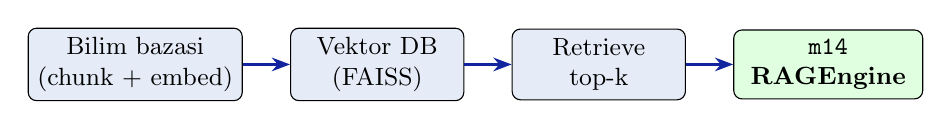
\begin{tikzpicture}[
      mod/.style={draw, fill=cnubluebg, rounded corners=3pt,
                  minimum width=2.2cm, minimum height=0.75cm,
                  font=\small, align=center},
      fin/.style={draw, fill=green!12, rounded corners=3pt,
                  minimum width=2.4cm, minimum height=0.75cm,
                  font=\small\bfseries, align=center},
      arr/.style={-{Stealth}, thick, color=cnublue}
  ]
    \node[mod] (kb) {Bilim bazasi\\ (chunk + embed)};
    \node[mod, right=0.6cm of kb]  (vs) {Vektor DB\\ (FAISS)};
    \node[mod, right=0.6cm of vs]  (re) {Retrieve\\ top-k};
    \node[fin, right=0.6cm of re]  (m14) {\texttt{m14}\\ RAGEngine};
    \draw[arr] (kb)--(vs); \draw[arr] (vs)--(re); \draw[arr] (re)--(m14);
  \end{tikzpicture}
  \end{center}
  \vspace{5pt}
  \begin{columns}[T]
    \begin{column}{0.50\textwidth}
      \textbf{P14 da qurasiz:}\\[3pt]
      \small
      \begin{itemize}\setlength\itemsep{2pt}
        \item \texttt{m14 RAGEngine}: chunk $+$ embed $+$ FAISS $+$ generate
        \item top-k retrieve va prompt yig'ish
        \item javobni kontekstga tayantirish
      \end{itemize}
    \end{column}
    \begin{column}{0.46\textwidth}
      \textbf{Birinchi assert (bu slayd [I2]):}\\[4pt]
      \small\ttfamily
      assert prompt\_tokens == 700\\
      assert retrieved\_docs == 3\\[4pt]
      \normalfont\footnotesize\color{halfgray}
      \textit{\# Ma'ruza L14 [I2]-slayd bilan}\\
      \textit{\# solishtiring (RAG token hisobi)}
    \end{column}
  \end{columns}
\end{frame}

% ----------------------------------------------------------------
% [R] ADABIYOTLAR
% ----------------------------------------------------------------
\begin{frame}{Adabiyotlar}
  \begin{enumerate}\small\setlength\itemsep{5pt}
    \item Lewis, P., va boshq.\ (2020). \textit{Retrieval-Augmented Generation
          for Knowledge-Intensive NLP Tasks.} NeurIPS 33.
    \item Karpukhin, V., va boshq.\ (2020). \textit{Dense Passage Retrieval for
          Open-Domain Question Answering.} EMNLP 2020.
    \item Johnson, J., Douze, M., Jegou, H.\ (2019). \textit{Billion-scale
          Similarity Search with GPUs (FAISS).} IEEE Big Data.
    \item Malkov, Y., Yashunin, D.\ (2018). \textit{Efficient and Robust ANN
          Search using HNSW.} IEEE TPAMI.
    \item \texttt{sentence-transformers} va \texttt{faiss} hujjatlari.
  \end{enumerate}
\end{frame}

% ================================================================
% [S] ILOVALAR (appendix --- slayd soniga kirmaydi)
% ================================================================
\appendix

\begin{frame}{Ilova S1: chunking strategiyalari}
  \small
  Hujjatni bo'laklarga ajratishning keng tarqalgan usullari:
  \begin{itemize}\setlength\itemsep{2pt}
    \item \textbf{Sobit hajm}: har $N$ token (oddiy, ammo gapni kesishi mumkin).
    \item \textbf{Gap/paragraf bo'yicha}: mazmunan to'liq, tabiiy chegaralar.
    \item \textbf{Overlap bilan}: bo'laklar biroz ustma-ust --- chegaradagi
          kontekst yo'qolmaydi.
  \end{itemize}
  \bunda{O'zbek huquqiy matnida modda/band bo'yicha bo'lish ko'pincha eng mosi
  --- har bo'lak mustaqil ma'noga ega bo'ladi.}
\end{frame}

\begin{frame}{Ilova S2: HNSW indeksi (qisqacha)}
  \small
  HNSW (Hierarchical Navigable Small World) --- ANN uchun ko'p qatlamli graf:
  \begin{itemize}\setlength\itemsep{2pt}
    \item Yuqori qatlamlar --- siyrak, uzoq "sakrashlar" (tez yo'naltirish).
    \item Quyi qatlamlar --- zich, aniq qo'shnilar.
    \item Qidiruv yuqoridan boshlanib, pastga "tushadi" --- $\approx O(\log n)$.
  \end{itemize}
  \bunda{Aniqlik/tezlik almashinishi \texttt{ef} va \texttt{M} parametrlari bilan
  sozlanadi --- katta \texttt{ef} aniqroq, ammo sekinroq.}
\end{frame}

\end{document}
